\chapter{La composante stellaire}


Maintenant que nous avons survolé toutes les physiques a l’œuvre dans ce type de simulation, concentrons nous sur les sources lumineuse.
comme nous avons vu, il existe deux types de sources, les étoiles et les quasars. %TODO ref
Je n'ai considérer que la partie stellaire.

L'objectif de cette section est d'exposer le modelé stellaire que j'ai développé.
Nous allons définir les différentes phase de la vie d'une étoile, et ses différentes évolution possible.
Nous verrons qu'elles sont les contraintes imposées par la résolution des simulations cosmologique.



\section{Les différentes phases de la vie d'une étoile}


définition d'une étoile


\subsection{Naissance}

%lien avec la densité\\
%Formation dans l'H moléculaire mais pas dans les simu

En principe une étoile se forme par effondrement gravitationnel.
Dans un nuage, si le temps de chute libre est supérieur au temps de rection a une perturbation le milieu n'a pas le temps de résister a son effondrement et le gaz s'effondre sur lui même.
Cette ne s’arrête que quand les réaction thermonucléaire s'enclenche et que le gaz forme une étoile.

Il y a effondrement si:
\begin{equation}
t_{ff} < t_{sound},
\end{equation}

avec:
 
\begin{equation}
t_{ff} = \frac{1}{\sqrt{G \rho}},
\end{equation}

et 

\begin{equation}
t_{sound} = \frac{R}{C_s},
\end{equation}

Ici intervient la densité, plus le milieu est dense plus il aura tendance a s'effondrer sur lui même.
D'un autre coté intervient aussi la vitesse du son $C_s$, elle même dépendante de la température $C_s \propto \sqrt{T}$.
Plus le gaz sera chaud, plus le nuage devra être gros pour pouvoir s’effondrer.



\subsection{Population III}

%tres peu de ligne de refroisdissment
%étoiles plus grosse
% temps de vie court

Or a haut redshift, au moment de l'apparition des premières étoiles, les métaux étaient trés peux disponible (cf nucléosynthèse primordiale) %TODO ref
De ce fait, le gaz disposait de relativement peu de possibilité de refroidissement, et donc la température du gaz devait être élevée.
Les étoiles primordiales devaient donc être plus grosses que les étoiles de notre voisinage (plus de 100Mo).
Ce type d'étoiles est appelées étoiles de population III.
Du fait de leur masse, elles émettait un fort rayonnement ionisant, et avaient une vie relativement courte.



%La nucléosynthèse primordiale a créer peu de métaux. 
%A haut redshift, les metaux etaient peu disponible.
%les métaux permettent une meilleur emmission radiative, et donc un meilleur refroidissent.
%si le refroidissment est meilleur, l'equilibre hydrostatique penche an faveur de plus grosse étoiles.
%POPIII, IMF top Heavy, étoiles  primordiales
%
%plus un étoiles est grosse, plus son spectre sera énergétique et plus la portion de spectre ionisant sera important.



\subsection{sequence principale}

%le diagram HR


Une fois le nuage de gaz effondré et les réaction thermonucléaire amorcées.
l'étoiles amorce sa séquence principale.
C'est la phase qui représente la majore partie de la vie d'une étoile.
Elle consiste en un équilibre hydrostatique entre gravitation et réaction de fusion nucléaire nucléaire.

%develloper le cycle proton proton ?
Équation simplifié du processus de fusion:
\begin{equation}
4p \leftrightarrow He^4 + 2e+ + 2\nu + E
\end{equation}

L'étoile va donc consommer son hydrogène pour résister a l’effondrement gravitationnel.
Il en résultera la formation d'hélium.

Plus une étoile est grosse plus le taux de réaction doit être élevé pour lutter contre la gravité.
Il en résulte que les grosse étoiles sont plus énergétique, et emmetent donc plus de rayonnement ionisant.
Mais ce taux de réaction élévé mêne a une durée de vie plus courte.

%materiaux de base est l'hydrogene\\
%plasma donc hydrogène ionisé 

\subsection{mort}

Arrivé a un certain taux de consommation d'hydrogène, 
les réactions ne sont plus suffisante et l'étoile s’effondre.
En fonction de sa masse, plusieurs scénario d’évolution sont possibles:


%Consomation du materiaux de base

géante rouge\\
naine blanche\\
trou noir\\
supernovae\\
formation d'elements lourd (>Fe)
enrichissement du milieu







A la fin de se vie, une étoile a consommée la plus grande partie de son hydrogène disponible.
l'équilibre radiatif est rompu et l'étoile s'éffondre.
cette augmentation de la pression amorce une serie de fusion nucléaire d’élément plus lourd que l’hydrogène.
cycle CNO
Une fois arrivé au Fe, il devient coûteux de continuer a fusionner.
FE le plus stable



Géante rouge

En fonction de la masse:
naine blanche (pression de dégénérescence des électrons)
étoile a neutron (pression de dégénérescence des neutrons)
trou noir (singularité)



Différents type de supernovae

I -> binaire accrétante du compagnon -> passage au dessu de la limite.
II -> l'étoile est assez massive au départ (M>8Mo)


Les supernovae ont été introduite dans les simulations cosmologiques pour contre ballancer "l'overcooling probleme".
Sans l'introduction d'énergie dans le gaz par les supernovae, le gas s'éffondre de manière importante et créer un nombre élevé d'étoiles.
cela mène a un taux de formation stellaire trop important par rapport a ce qui est observé.



les superbubbles
A la manière de la percollation des bulles de HII, les bulles de supernovae 





\section{Population stellaire et modèle sous grille}

\subsection{Problème de résolution}

%En fonction des echelles de travail, nous considererons soit les etoiles individuelles soit une population stellaire.


Une des difficulté des modèles stellaire dans les simulations de réionisation, et le manque de résolution.
Il existe toujours ce conflit en réionisation entre simuler des grands volume, et obtenir la meilleur résolution possible.
Actuellement les simulations les plus résolues et capable de suivre un volume d'Univers suffisant atteigne un résolution de l'ordre de la centaine de parsec.
Or les échelles de formation stellaire sont de l'ordre de l'unité astronomique, soit un facteur $\approx 10^6$ plus petit.
Il n'est donc actuellement pas possible de suivre la formation des étoiles individuellement.

Il nous faut créer un modèle qui va tenter de prendre en compte au mieux la physique non résolue.
Ce type de modèle est appelé modèle sous grille.

Dans le cas présent le modèle sous grille consiste a transformer une partie du gaz en particule stellaire.
On appelle ces particules des particules puits.
Toute la difficulté du modèle de formation stellaire sera de déterminer la façon dont est réalisée cette conversion.
Malgré tout, nous verrons qu'il est possible d'obtenir un modèle statistiquement viable a grandes échelles assez facilement.

Un second type de modèle intervient au moment de l'explosion en supernovae.
Les processus de diffusion de l'énergie libérée aux échelles plus petite que la grille sont complexe et il en résulte une série de paramètres libres assez conséquente.

%lien entre les différents solveurs en fonction du stade évolutif
Les étoiles se trouvent aux centre de la simulation.
En effet, créer une étoiles consiste a transformer une partie du gaz en particule.
Cette particule sera ensuite gérée par le solveur Ncorps, et servira de source au solveur radiatif.
Puis a la fin de sa vie, l'étoile va injecter de l'énergie dans le solveur hydrodynamique.
Une particule stellaire va donc devoir interagir avec tout les solveurs du code.




%Seul la partie du spectre capable de ioniser l'hydrogène est considérée. E>13.6eV



\subsection{Fonction de masse Initiale}

Les étoiles naissent en groupe.
La probabilité de former une étoile d'une certaine masse est régie par la fonction de masse initiale (IMF)
Il existe différentes IMF, parmi les plus connues il y a :

\begin{itemize}
\item \cite{1955ApJ...121..161S}
\item \cite{1979ApJS...41..513M}
\item \cite{2001MNRAS.322..231K}
\item \cite{2003PASP..115..763C}
\end{itemize}

Comme nous l'avons abordé plus haut, les étoiles de population III avaient tendence a être tres massive.
De plus, certain travaux (eg \cite{2003MNRAS.344L...7C} ) sugère une IMF top heavy, c'est a dire une IMF avec une proportion d'étoile massive très importante.
La majorité des simulations que j'ai réalisées utilisent une IMF Top-Heavy.

J'ai commencé mes calibrations avec une IMF de Salpeter, mais il s'est vite avéré que les sources n’émettaient pas assez de photons et que les boites n'arrivaient pas a reioniser
%: difficulté a reioniser avec Salpeter -> passage a top heavy -> justification 
%Fonction de masse IMF Top Heavy


\subsection{Starburst99}

%Pour modeliser 
%paramètre d'entrée
%sorties

La modalisation de population stellaire est complexe, et il existe différent modèles complets.
J'ai choisi d'utilisé Starburst99 \citep{leitherer_starburst99:_1999} mais il en existe d'autres : \cite{2003MNRAS.344.1000B} , FSPS \cite{2009ApJ...699..486C}.  
%TODO mettre les differnts models

A partir d'information caractéristique d'une population stellaire, comme sa masse, son IMF ou sa métallicité, Starburst99 retourne le spectre d'émission de cette population en fonction du temps cf (Fig \ref{fig:spectre_starburst}).

\begin{figure}[htbp]
        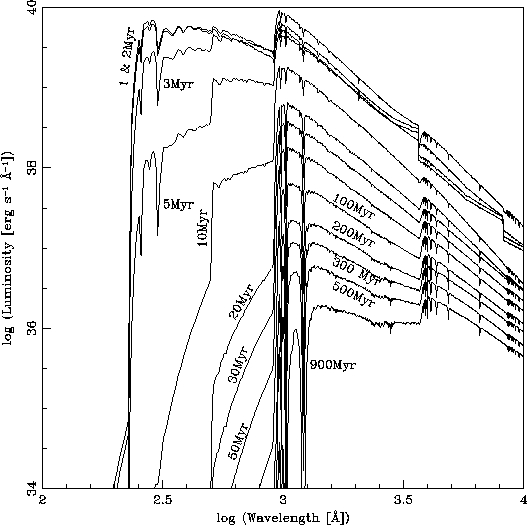
\includegraphics[width=.95\linewidth]{img/03/spectre_starburst.jpg} 
        \caption{Spectre d'émission d'une population stellaire généré par Starburst99.
        Ici avec les paramètres M=1e6 Mo, IMF de Salpeter ($\alpha=2.35$ et intégration de 1 a 100 M$_\odot$ }
 		\label{fig:spectre_starburst}
\end{figure}

Un avantage de Starburst99 par rapport a d'autre modèle et qu'il retourne également de l'information utile pour la modélisation des supernovae.
Nous y reviendrons dans la section dédiée. %TODO ref


\section{La formation stellaire}

\subsection{Localisation des zones de formation stellaire}

Il est admis que les étoiles se forment dans les nuage moléculaires.
Ces nuages ce trouvent eux meme dans des zones suffisement dense pour que les molecules puissent se former.
En pratique dans EMMA, 
%la physique de l'hydrogene moléculaire n'est pas prisent en compte 
Les zones capables de former des étoiles sont localisées a l'aide d'un seuil en densité.
Toutes les cellules en dessous d'un certain seuil ne sont pas authorisée a créer des particules stellaire.

%Seuil en densité \\
\begin{equation}
	flag = 
  \begin{cases}
      True, & \text{if } \rho > \rho_{thresh}\\
      False,              & \text{otherwise}
  \end{cases}
\end{equation} 

Cette densité de seuil $\rho_{thresh}$ peux être définie arbitrairement.
Comme toute densité, elle est dépendante de la résolution.
De plus il en possible de définir une densité en unité physique ou en unité commobile.
Un seuil en densité physique sera plus représentatif de se qui se passe réellement.
Mais a haut redshift, la densité était haute partout, et un seuil en unité comobile est utile pour limité l'aparition des premières étoiles a un redshift donné.
%TODO figure du seuil en fonction du redshift
En pratique on pourra définir ces deux seuil, et le seuil final sera le plus contraignant des deux.

\begin{equation}
	\rho_{thresh} = max\left(  \delta_{in} \bar{\rho}, \rho_{in} a^3 \right)
\end{equation} 

ou $\delta_{in}$ et $\rho_{in}$  sont respectivement les paramètre de surdensité et de densité physique.
$\delta_{in}$est exprimé en unité comobile et est donc constant dans le temps en unité du code
 $\rho_{in}$ est exprimé en unité physique (en atome par metre cube), sa valeur evolue dans le temps du point de vue des unité du codes.

% determination de la valeur de 55\\ 



\subsection{La loi de schmidt-kennicut}
 %conversion densité surfacique vers densité 3D\\
%rho 1.5\\
%temps de free fall\\

Maintenant que nous avons définis ou former des étoiles, il faut calculer combien nous devons en former.

La loi de Schmidt %TODO ref
est une loi observationnelle qui lie la densité surfacique de gaz dans les galaxies au taux de formation stelaire (SFR) dans cette galaxie.
Kennicut %TODO ref
a utilisé un model de galaxie pour dé projeté la densité surfacique observé et ainsi determiner une loi qui lie le SFR a la densité volumique de gaz.

Il est arrivé a une loi de la forme:
\begin{equation}
SFR \propto \rho ^{\alpha}
\end{equation}

avec $\alpha \approx 1.5$

 
Le taux de formation stellaire s'exprime généralement en $M_\odot \cdot Mpc^{-3}  \cdot yr^{-1}$  
Ce qui est homogène a une densité divisé par un temps.


En pratique divisera $\rho_g$ la densité de gaz locale par le temps de chute libre ,
\begin{equation}
t_{ff} = \sqrt{\frac{3\pi}{32G\rho_g}}.
\end{equation}

Ce qui nous mène a considérer, dans les cellules autorisée, une SFR sous la forme:

\begin{equation}
	SFR = \epsilon_{sf} \frac{\rho_g}{t_{ff}}
    \label{eq_sfr}
\end{equation}

avec  $\epsilon_{sf}$ le paramètre d'efficacité de formation stellaire.
Observationellement, $\epsilon_{sf}$  est de l'ordre du \%. %TODO ref
Ce qui signifie que la formation stellaire est relativement inéfficace.
Utiliser le temps de chute libre dans cette expression fait sens puisque en théorie c'est le temps qu'il faudrait a un nuage de gaz pour s'effondrer si il n'y avait aucune resistance.
En pratique le temps caractéristique de formation stellaire:
\begin{equation}
t_{sf} =  \frac{t_{ff}}{ \epsilon_{sf} },
\end{equation}
est de l'ordre de quelques milliard d'années.

A partir de ce taux de formation on obtient la masse de gaz a convertir en étoile dans chaque cellule en multipliant par $dv$ le volume de la cellule en question et $dt$ le pas de temps entre deux passage dans la fonction de formation stellaire.

\begin{equation}
	M_{star} = SFR . dv .dt 
\end{equation}

%resolution en masse\\

Nous avons donc a ce stade la masse totale de gaz a convertir en étoile.
Il devient rapidement couteux de générer pour chaque cellule éligible, et a chaque pas de temps, une nouvelles particule stellaire (le nombre de particule peux rapidement exploser.
Nous adoptons une approche probabiliste.
Nous définissons une masse d'étoiles $m_{star}$ qui correspondra a notre "quanta stellaire".
toutes les étoiles aurons donc la même masse.
La masse des étoiles est calculée d'une manière comparable a la masse d'une particule de matière noire.
la masse d'une étoile correspond a la masse moyenne de gaz dans une cellules d'un certain niveau pouvant aller du niveau coarse $m_star = M_{DM} \frac{\Omega_b}{\Omega_m}$ au niveau plusieurs niveau raffiné.


Et nous tirons le nombre de quanta a ajouter aléatoirement dans une lois de Poisson.

\begin{equation}
	P(N) = \frac{\lambda^N}{N!} e^{-\lambda}
\end{equation}

Ou $\lambda$ correspond au nombre de particule moyen a créer dans la cellule :
\begin{equation}
\lambda = \frac{ M_{star}}{m_{star}}
\end{equation}
Étant donné le grand nombre de tirage cette loi est en moyenne valide.
On obtiendra au final $N_{star}$ le nombre de quanta de masse d'étoile a créer.


En pratique j'ai implémenté deux méthodes de transformations.
Si  $N_{star}>1$ il est possible de créer : 
\begin{itemize}
\item  $N_{star}$ particules aillant chacune une mass  $m_{star}$.
\item une seule particule de masse  $N_{star} \cdot m_{star}$.
\end{itemize}

Dans le premier cas le nombre de particules sera plus élevée et la résolution stellaire meilleure, mais en contrepartie le cout numérique sera plus important.
Le choix de la méthode est laissé a l'utilisateur.

En pratique la création d'une particule stellaire consistera a 
\begin{itemize}
\item prendre dans la réserve, une nouvelle particule %un maillon de la liste chainée
\item ajouter ce nouveau maillons a la liste chainée de particule de la cellule.
\item initialiser cette nouvelle particule avec : 
\begin{itemize}
\item un état
\item un temps de création
\item une vitesse 
\item une masse
\item un identifiant
\end{itemize}
\end{itemize}


On associera un temps de création a la particule stellaire et non un age, ceci permet de ne pas avoir a remettre a jour cette valeur a chaque pas de temps.
Pendant les analyses post simulation, on prendra garde a définir l'age des étoiles comme étant le temps associé au snapshot courant moins le temps de création de la particule.

Les étoiles créées auront une vitesse aléatoire pour éviter les effets de "collier".


Il est utile d'associer un identifiant unique aux particules.
Cela permet de les retrouver entre les différents snapshot.
La technique la plus simple est d'associer la valeur d'un entier que l'on incrémente a chaque création d'une nouvelle particule.
Du fait de la parallélisation cette incrémentation est compliquée et demande des communications a chaque création de particule.
La pratique retenue consiste a former toutes les particules de toutes les processeurs, en leur assignant un identifiant caractéristique (ici -1) et d'assigner les identifiant finaux dans un second temps.
Une fois les particules créées,  on compte le nombre de nouvelles particules dans chaques processeurs.
Ce qui permet d'allouer une plage d'identifiants par processeurs, et ainsi allouer les identifiants finaux.


\section{le SFH cosmique}

Dans le but de tester cette implémentation, le premier test réalisé consiste a comparer la SFR cosmique de l'ensemble de la boite, aux observations.
Les points d'observations de Bouwens %TODO ref

%TODO mettre figure SFR qui passe dans les cloups.

Des test plus poussés seront développés plus loin.



\section{La vie radiative}
%injection d'énergie dans le solveur radiatif, ok mais combien?\\
%calibration energetique et Starburst99\\

Une fois les étoiles formées, il est nécessaire de les faire rayonner.
Pour ce faire il faut passer en revue toute les étoiles, et a partir de leurs masse et de leur age, calculer leurs émissivité.
Cette opération est simplifiée par l'utilisation de la liste chaînée de particule associées a chaque cellule. %TODO ref section
En effet, en pratique, on passera en revue toutes les cellules, et pour chaque cellules on passera en revue toutes ses particules.
On testera alors si une particules est une étoiles (la liste chainée contient également les particulke de matière noire), et si cette étoiles est dans un stade ou elle émet de l'énergie lumineuse.
Si c'est le cas, on calculera son émissivité et on injectera cette énergie sous forme de source dans l'équation \ref{eq:densite_energie}.
Le calcul de $\dot{N}_\nu^*$ sera effectué dans toutes les cellules.

La principale question a laquelle tente de répondre cette section est : Quel est le lien entre age, masse et luminosité d'une particule stellaire?
Pour répondre a cette question on utilisera un modèle de population stellaire.

A partir des spectres obtenus avec Starburst99, nous allons ne garder que la partie capable de ioniser l'hydrogène (toutes les longueurs d'onde plus petite que 911$\AA$) 

\begin{equation}
E_{ion} = \int_{13.6eV}^{+\inf} h \nu d\nu
\end{equation}

On obtient a partir de cette intégration, un profil de luminosité présenté sur la figure \ref{fig:flux}.

\begin{figure}[htbp]
        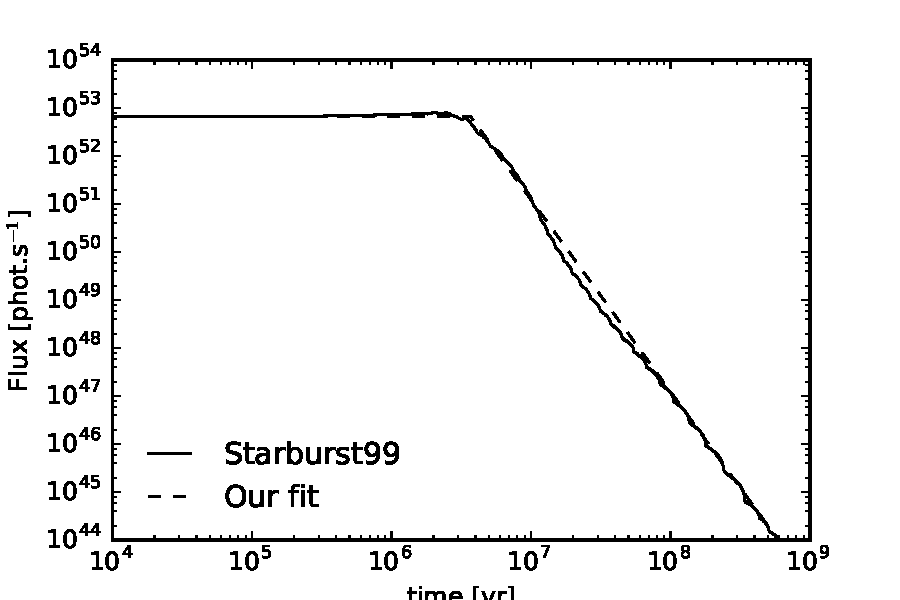
\includegraphics[width=.95\linewidth]{img/03/flux.pdf} 
        \caption{Émissivité ionisante intégrée en fonction du temps}
 		\label{fig:flux}
\end{figure}

Le profil obtenu présente un plateau d'émissivité constante suivie d'une rapide décroissance.
Ce profil peut être raisonnablement approximé par:

$
    S = 
\begin{cases}
    S_0 ,         & \text{if } t < t_{life}\\
    S_0.t^{-4},   & \text{if } t_{life} \leq t < 100.t_{life} \\
    0,   & \text{if } 100t_{life} \leq t
\end{cases}
$

Ce flux correspond au flux d'une population de $10^6M_\odot$.
Ces valeurs seront pondérées au prorata de la masse de la particule stellaire. (Une particule de $10^5M_\odot$ émettra 10 fois moins de photons).

Ce profil d’émission ionisante peut être découper en différents "groupe de photons" (cf section \ref{sec:groupedephotons}).
Il est possible de choisir un nombre arbitraire de groupes, mais il faut prendre en compte que chaque groupe devient l'équivalent d'un fluide dont on veut suivre l'évolution.
Le coût numérique augmente rapidement avec le nombre de groupes. 
J'ai implémenté la possibilité de découper les groupes, en fréquences, mais aussi en temps.
Malgré tout, le ratio cout de calcul sur amélioration des prédictions n'est pas en faveur de l'augmentation du nombre de groupes (dans le cas des résolution considérée pendant ma thèse).
En pratique on prendra un généralement un seul groupe de photons.

L’énergie moyenne d'un photon dans un groupe est calculée de la manière suivante:
\begin{equation}
<E> = \frac{1}{N} \int_{\nu_1}^{\nu_2} N_\nu h \nu d\nu
\end{equation}

et la section efficace d'intéraction:
\begin{equation}
\sigma_E = \frac{1}{N<E>} \int_{\nu_1}^{\nu_2} N_\nu h \nu d\nu
\end{equation}

Pour une IMF TopHeavy, les valeurs obtenues sont:


\begin{table}
\begin{tabular}{l l }
	$<h\nu>$	&  23.42 eV \\
	$\alpha_e$	&  $2.35.10^{-22}$ m$^2$ \\
	$\alpha_i$	&  $1.82.10^{-22}$ m$^2$ \\
\end{tabular}
\caption{Propriété des photon émis par les sources.
\label{tab_photon}}
\end{table}

La table \ref{tab_photon} présente les caractéristique des photons obtenus.


%TODO intégration de l'énergie et de la section efficace


%We found a mean energy of $<h\nu> = 23.42$ eV,
%an energy weighted cross section of
%$\alpha_e = 2.35.10^{-22}$ m$^2$
%and a number weighted cross section of
%$\alpha_i = 1.82.10^{-22}$ m$^2$


%Masse de la population\\
%produit en croix pour correspondre a la masse dans simu\\
%integration seulement sur energy ionisante\\
%
%Multigroupe frequence\\
%multigroup temporel\\


\section{le problème de la masse des étoiles}



%le paramètre de masse des étoiles change la reionization\\
%effet numérique\\
%le rayonnement est piégé dans les cellules\\

Durant mes calibrations, il s'est avéré que le paramètre de résolution de la masse des particules stellaire avait une grande importance dans l'évolution de la fraction ionisée.
Même si celui ci n'a pas d'impact sur la SFR globale, le taux d'ionisation moyen est fortement dépendant de ce paramètre.
Plus la résolution stellaire est élevée, plus la boite réionise tard.


%TODO ajouter les figures cf présentation pp




\section{Les supernovæ}


Les supernovae ont été introduite dans les simulations cosmologiques pour contre balancer "l'overcooling problem".
Sans l'introduction d'énergie dans le gaz par les supernovæ, le gaz s'effondre de manière importante et créer un nombre élevé d'étoiles.
cela mène a un taux de formation stellaire trop important par rapport a ce qui est observé.



\subsection{Le modèle théorique}
il existe principalement deux événement pouvant mener a un explosion de supernovæ : 

\begin{itemize}
\item soit l'étoile est a l'origine suffisamment massive (plus de 8Mo) pour s'effondrer a la fin de sa vie.
\item soit l'étoile n'est pas suffisamment massive (elle va donc mourir en naine blanche) mais dispose de suffisamment de matière a proximité (généralement étoiles double ou le compagnon pas en phase géante rouge) pour que sa masse augmente avec le temps.
la matière accreté va faire passer la masse de cette étoile au dessus de la limite.
\end{itemize}

Les étoiles de plus de 8mo exploses en SN en injectant 1e51 erg dans le milieu\\
Cette injection limite fortement la formation stellaire dans le milieu.\\
modèle sous grille\\
 
\subsection{Les différentes phases}

\begin{itemize}
\item Expansion adiabatique.
Dans la phase d'expansion adiabatique, l'énergie est conservée, le choc est violent et le gaz n'a pas le temps de perdre de l'énergie par radiation.
Dans cette phase, l'expansion est suffisamment rapide pour que la dissipation d'énergie par radiation soit négligeable.
C'est le cas dans le test de Sedov.

\item Snowplow.
Dans la phase snowplow, le choc a suffisamment ralentis pour que le gaz commence a rayonner de l'énergie, l'énergie n'est plus conservée.
Dans ce cas, il se forme un bourrelet de compression dans lequel le gaz est poussé, comme dans le cas d'un chasse neige. 
Les pertes par radiation deviennent importantes. 
\end{itemize}

\subsection{les superbubles}

%A la manière de la percolation des bulles de HII, les bulles de supernovae 

Dans les endroits de formation stellaire, les étoiles ne sont pas isolées mais apparaisent ensemble au sein d'un même nuage de gas.
L'effondrement gravitationnel du nuage mêne a créer un génération d'etoile en un cours laps de temps.
Toutes ces étoiles vont mourrir dans un laps de temps rapproché et ainsi, les differentes supernovae vont injectée de l'energy dans le milieu dans un temsp tres rapproché.
Les différentes bulle vont se rencontrer (a la manière des bulles ionizées) en mener a une bulle plus grande appelée superbuble.


\subsection{les considérations d'échelles}
La façon de gérer les supernovae sera donc fonction de l'échelle que l'on considère.
Dans des simulations très détaillées de galaxies, il sera nécessaire de résoudre la phase adiabatique d'explosion individuelle.
Dans des simulations cosmologiques de la reionisation, l'interet sera plus porté sur la phase snowplow des superbubbles.


\subsection{ Différentes implémentations existantes}



\subsubsection{Navaro and white}


\subsubsection{Stinson et al}



\subsubsection{dubois et Teyssier}

Utilisation de particule fantômes pour simuler les différentes phase

\subsubsection{Dalla Veccia et Schaye}

Modèle probabiliste, injection d'énergie seulement si l'énergie est suffisante pour générer un mouvement suffisant.


\subsection{Mes Implémentations}


\subsubsection{le model thermique}
Le modèle thermique consiste a injecter l'energie sous forme d'energie interne.
Il existe 2 variables d'etat liées a l'energie interne: la pression et la température.
Modifié l'une de ses 2 variables est equivalent.

Dans l'implementation actuelle, la pression est modifiée en utilisant cette conversion:

\begin{equation}
P^{0+} = P^{0-}  + E_0 * (\gamma-1)
\end{equation}

Ce modèle est connu pour avoir de fortes pertes de d'énergie dans le cas ou le refroidissement est autorisé.


\subsubsection{le model cinetique}


Le modèle cinétique consiste a modifier directement la vitesse du gaz autour de l'explosion dans le but de shunter la conversion de l'énergie interne en mouvement.
Ce type de model a été utilisé pour 

Nous avons fait le choix de limiter le nombre de cellules utilisées a 8 correspondant a 1 oct de la structure AMR d'\emma

\begin{equation}
e_{SN} = E_{SN}/8
\end{equation}

Ensuite cette énergie est utilisé pour changer la vitesse du gaz en utilisant : 
\begin{equation}
    \Delta \overrightarrow{v_{gas}} = \sqrt{\frac{2e_{SN}}{\rho_g.dV}} \overrightarrow{u}
    \label{eq_sn_direct}
\end{equation}


\subsection{Test numérique (Sedov)}

%la dérivation des solutions du test de Sedov se trouve :
%chapitre 17 de Shu the physique of astrophysic Volume 2.\\

Dans le but de tester l'implémentation des différents modèles d'injection d'énergie, je l'es ai soumis au test de Sedov.
Ce test est utilisé pour tester le cas d'une explosion parfaite.
Il consiste a relâcher instantanément une quantité d'énergie $E_0$ dans un milieu homogène d'indice adiabatique $\gamma$, de densité $\rho_0$ et de pression $P_0$ (ou de température $T_0$).
Ce brusque changement dans l'état du système créer une discontinuité que le solveur va devoir gérer.

L'avantage de ce test est qu'il dispose d'une solution analytique.
Sedov a exprimé  en 1959 que le rayon de l'explosion en fonction du temps peux s'exprime : %TODO ref

\begin{equation}
r_{(t)}=\left( \frac{E_0}{\alpha \rho_0 }\right)^{1/5} t^{2/5}
\end{equation}


\subsubsection{Sedov évolution temporelle }


parametre du test :
rho=1
p=1e-5
v=0
gamma=5/3


Ce test consiste a suivre l'onde de choc et a s'assurer que son profil et sa position sont correct dans le temps.
On calcul pour chaque cellule sa distance au centre de l'explosion, puis en utilisant un histogramme sur les rayons, pondéré par la valeur du champ que l'on veux analyser, on obtient rapidement le profil radial moyen.
Le résultats présentés utilise l'injection thermique simple (dans une seule cellule).

Le domaine de calcul est en une grille régulière décomposé en $256^3$ éléments  de calcul et le raffinement n'est pas autorisé.

La Fig. \ref{fig:sedov_evol} présentes le trois principaux champs (densité, pression et vitesse radiale) a trois instant différents, comparé a la solution analytique.
On observe un très bon accord en la simulation et le théorie.
Notre méthode d'injection d'énergie est correcte et bien dimensionnée.
%
%\begin{figure}[bth]
%        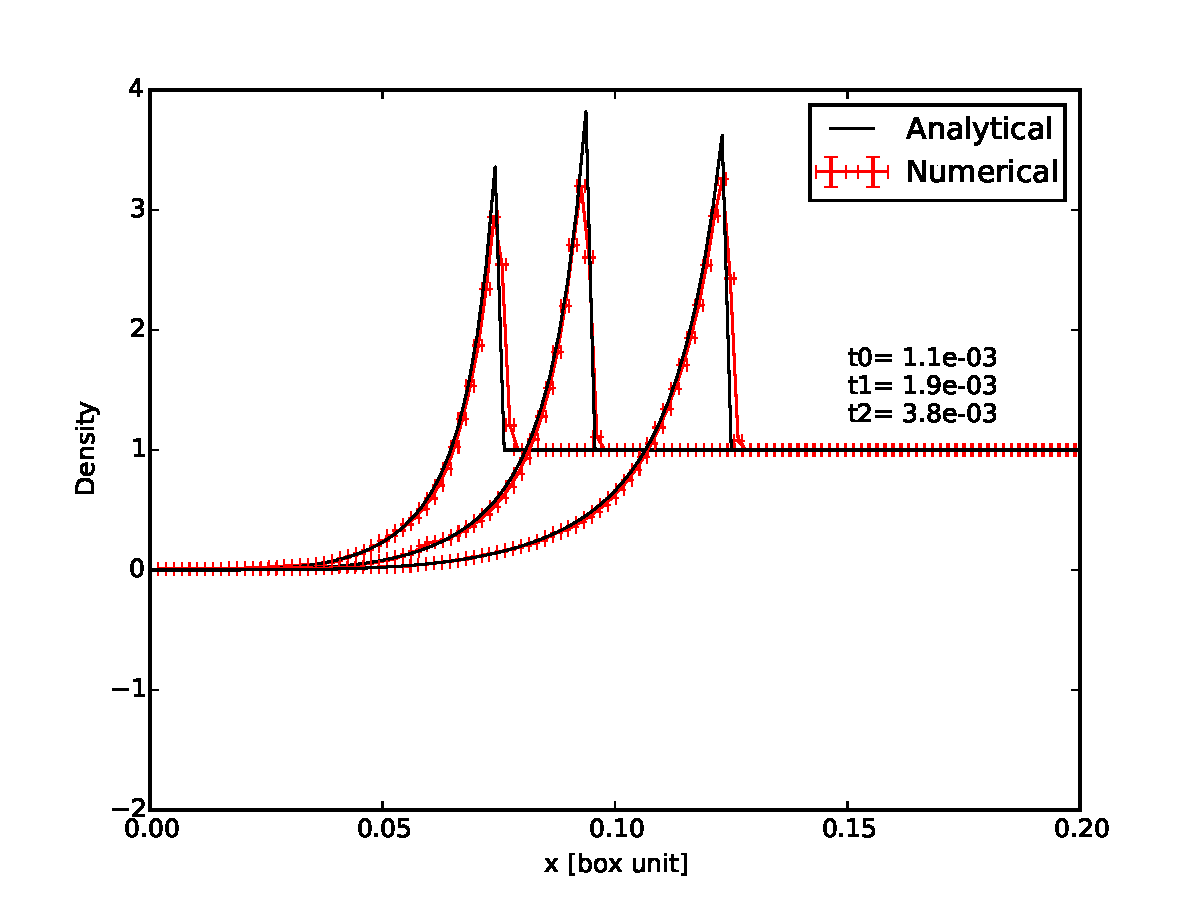
\includegraphics[height=.3\textheight]{img/03/sedov/sedov_evol_8_den_lin.pdf} 
%		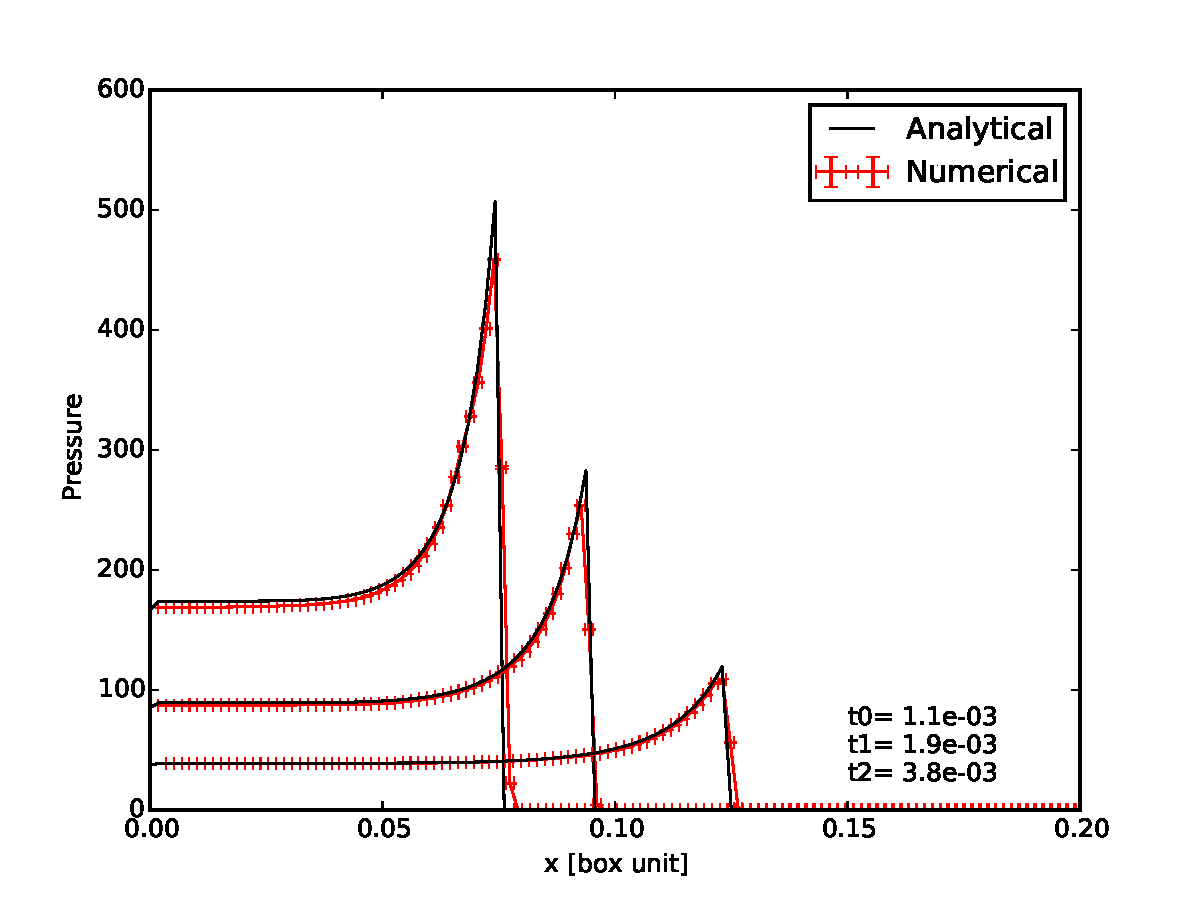
\includegraphics[height=.3\textheight]{img/03/sedov/sedov_evol_8_pres.pdf} 
%		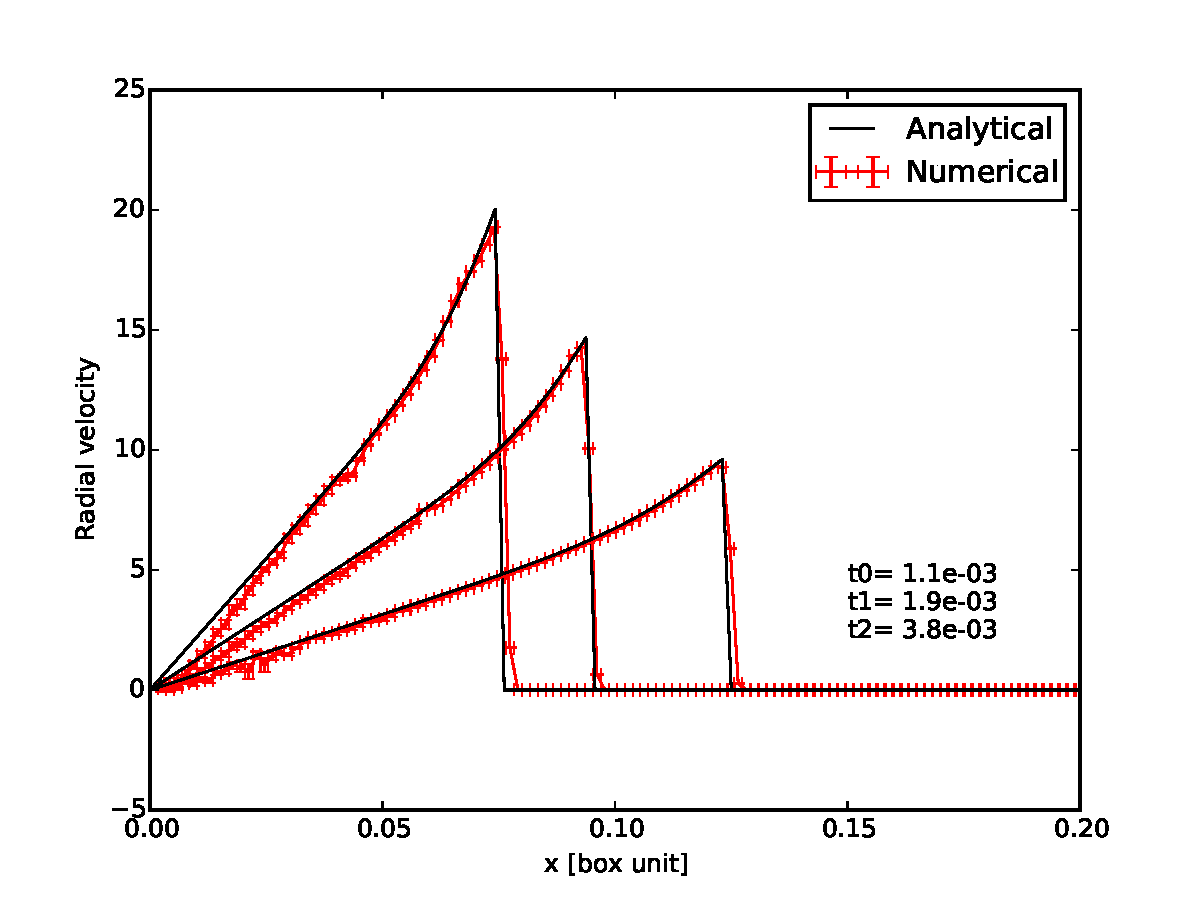
\includegraphics[height=.3\textheight]{img/03/sedov/sedov_evol_8_vel.pdf} 
%        \caption{Test de Sedov, évolution des différentes variables d'états. La densité en haut, la pression au milieu et la vitesse radiale en bas.}
% 		\label{fig:sedov_evol}
%\end{figure}

\begin{figure}[bth]
   \begin{minipage}[c]{.46\linewidth}
        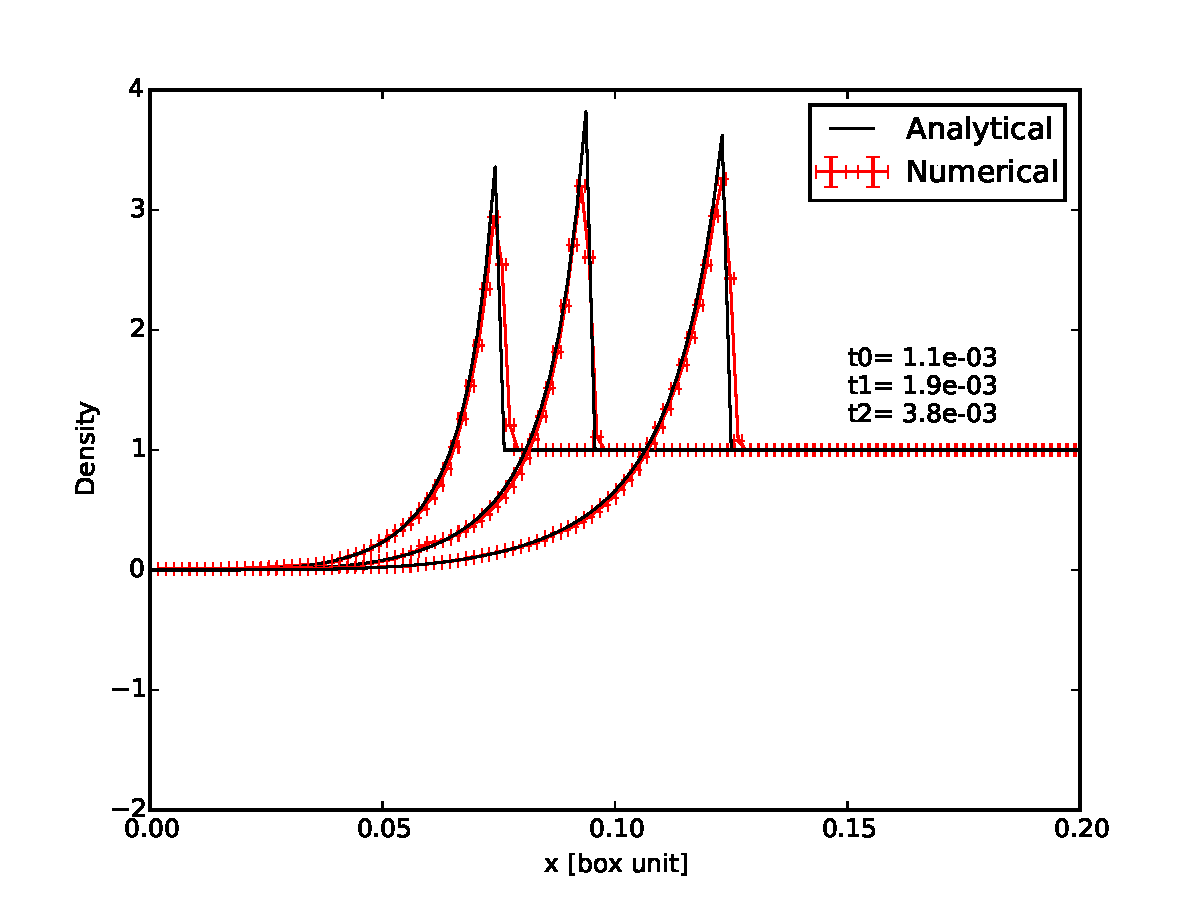
\includegraphics[width=\textwidth]{img/03/sedov/sedov_evol_8_den_lin.pdf} 
		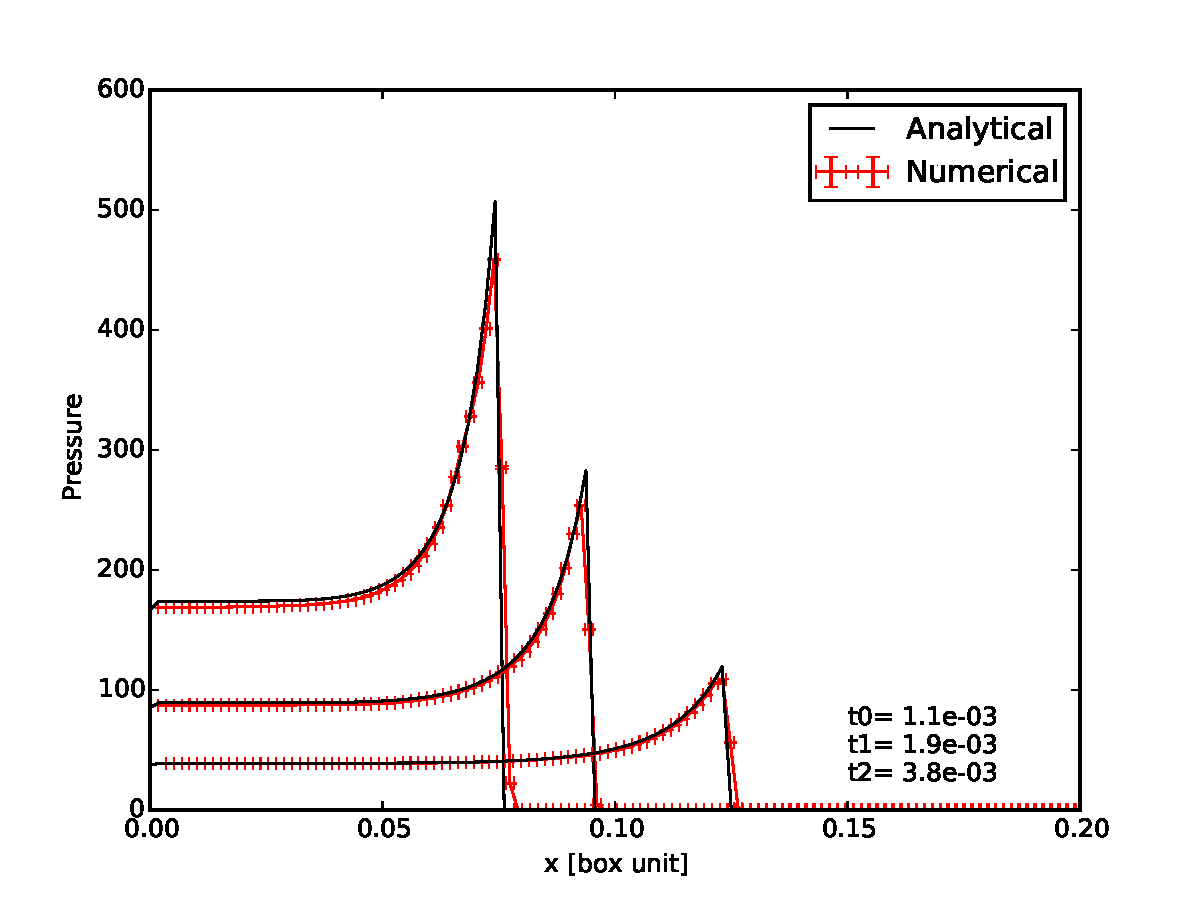
\includegraphics[width=\textwidth]{img/03/sedov/sedov_evol_8_pres.pdf} 
		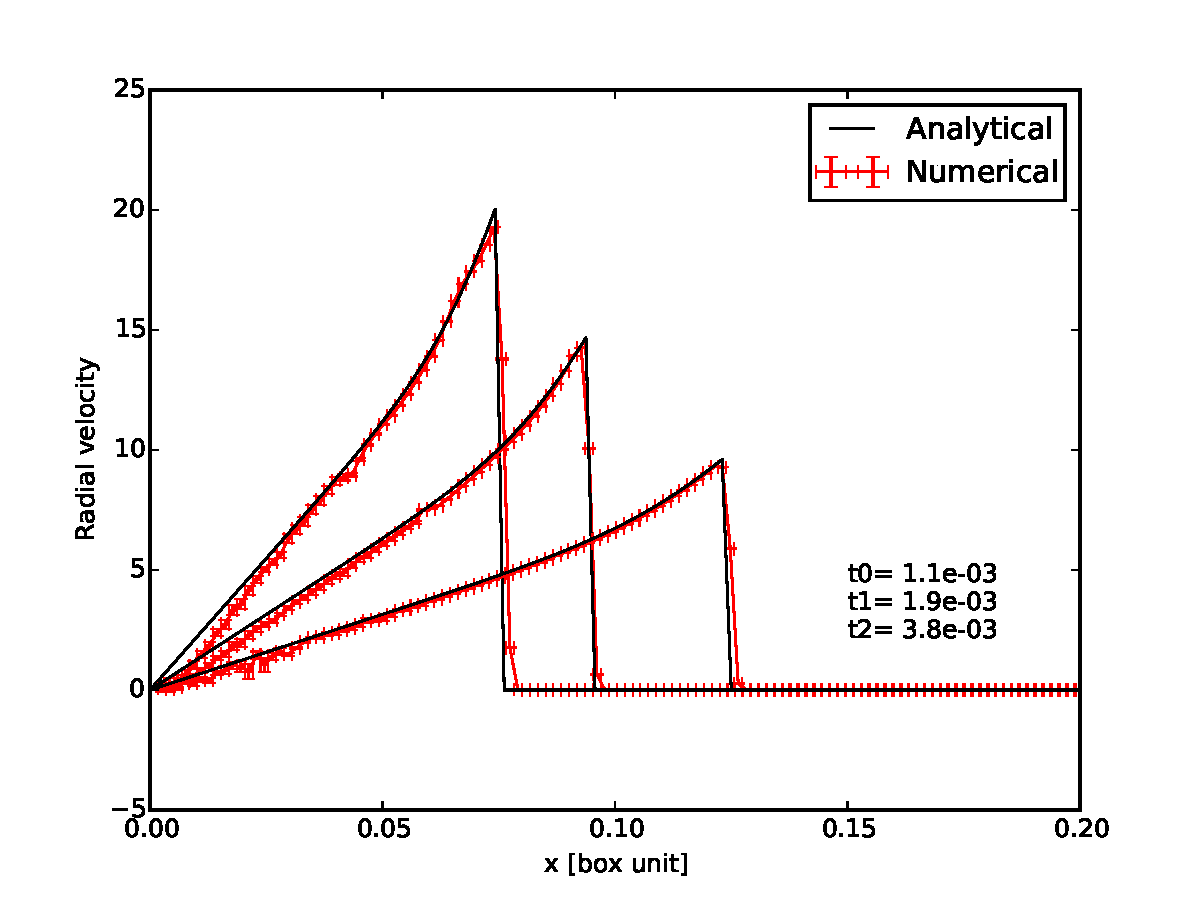
\includegraphics[width=\textwidth]{img/03/sedov/sedov_evol_8_vel.pdf} 

   \end{minipage} \hfill
   \begin{minipage}[c]{.46\linewidth}
		
		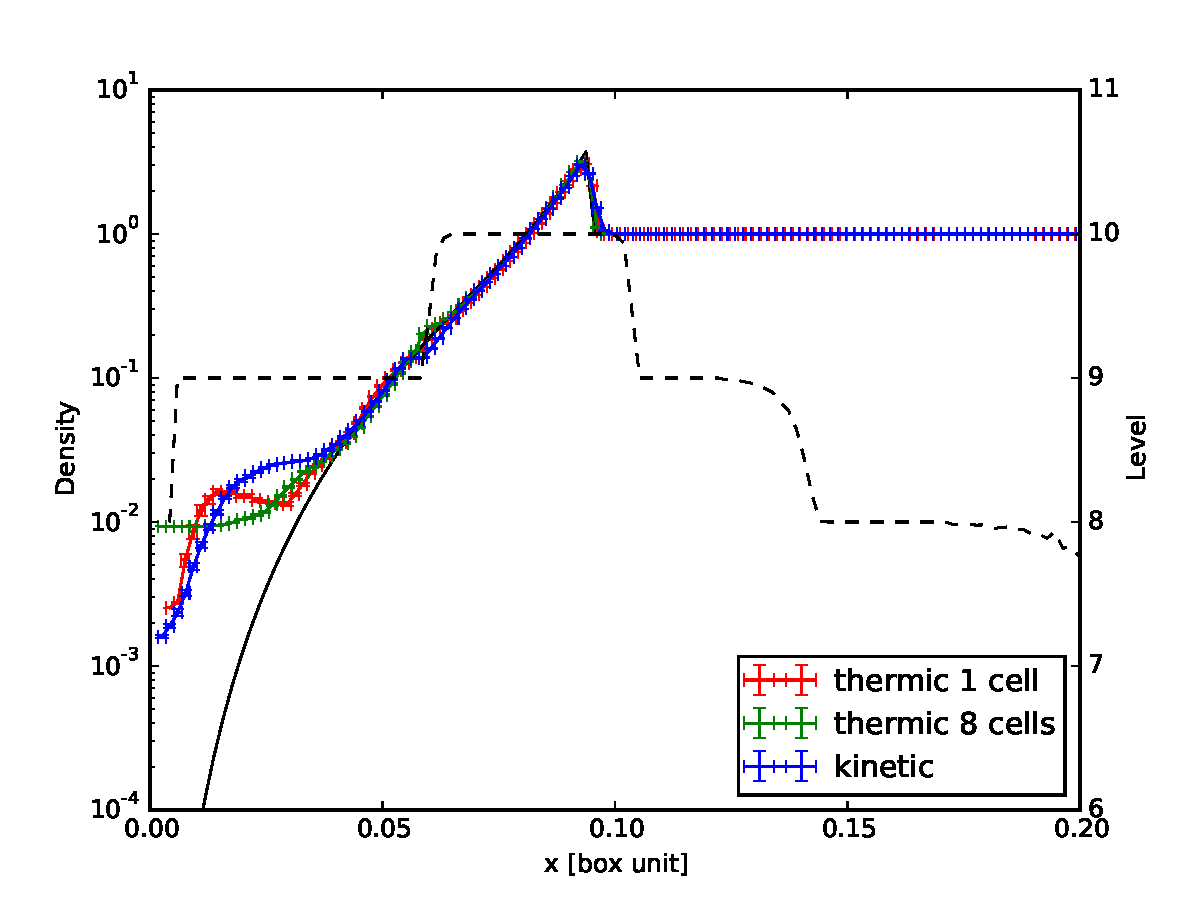
\includegraphics[width=\textwidth]{img/03/sedov/sedov_comp_profile_den.pdf} 
		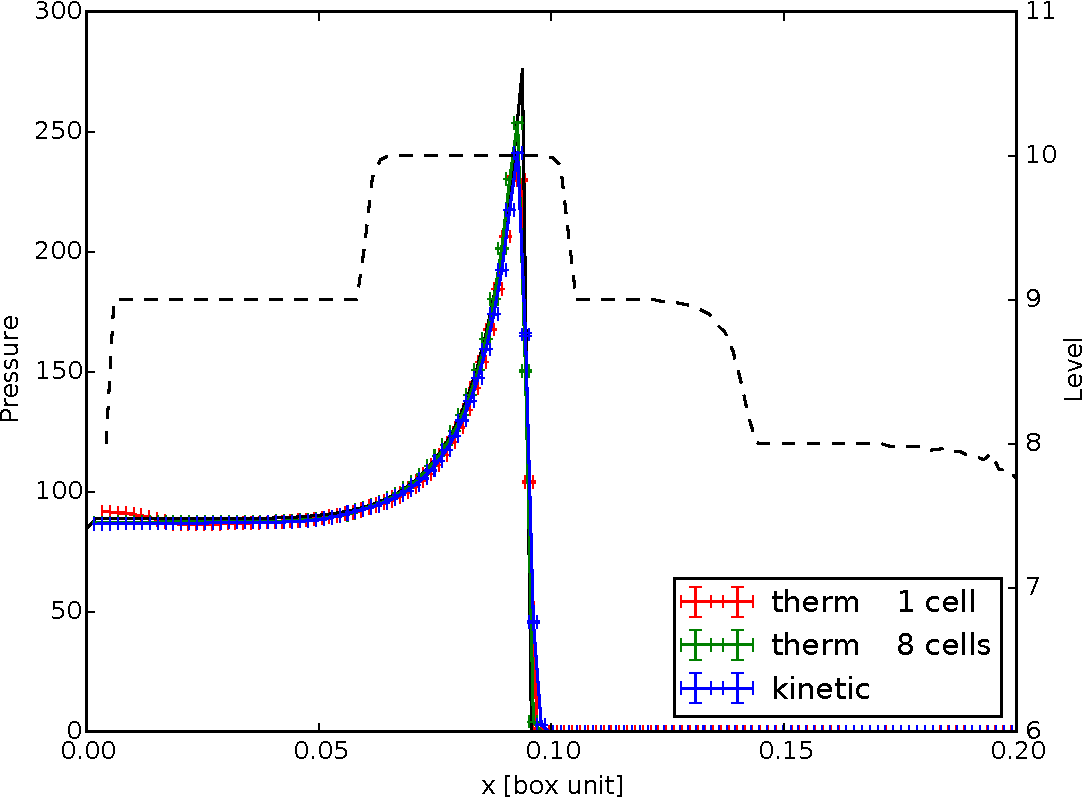
\includegraphics[width=\textwidth]{img/03/sedov/sedov_comp_profile_pres.pdf} 
		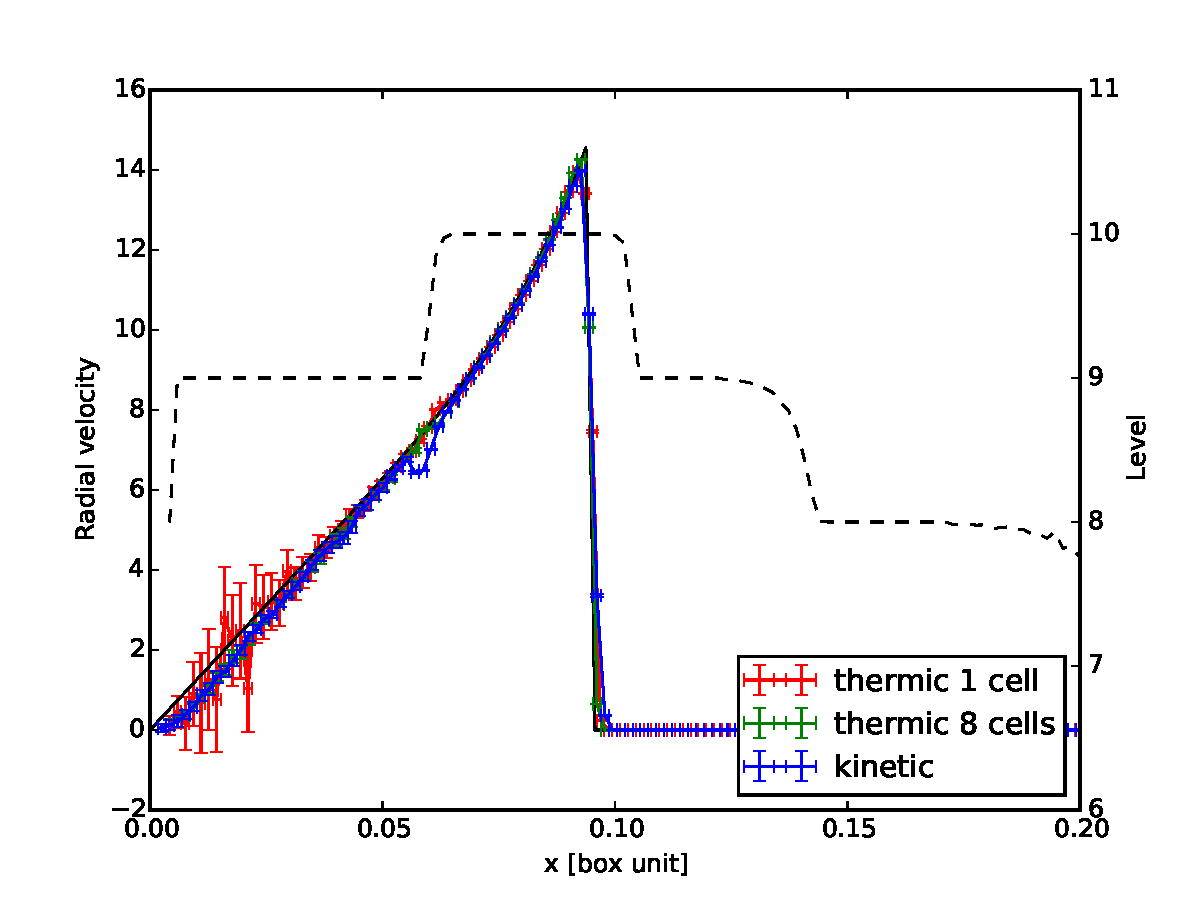
\includegraphics[width=\textwidth]{img/03/sedov/sedov_comp_profile_vel.pdf} 

   \end{minipage}

        \caption{Test de Sedov, évolution des différentes variables d'états. La densité en haut, la pression au milieu et la vitesse radiale en bas.        
        Test de Sedov, comparaison des profil radial en fonction des  méthodes d'injection. 
        Densité en haut, pression au milieu et vitesse radial en bas.
        La position et la forme du front d'onde ne dépendent pas de la méthodes d'injection utilisée.
% 		\label{fig:sedovmethod} 
 		}
 		\label{fig:sedov_evol}
\end{figure}



\subsubsection{Sedov comparaison entre les méthodes}

Nous avons vu qu'il existe différents moyens d'injecter de l'énergie dans le solveur hydrodynamique.
Le test présenté ici consiste a vérifié que les différentes méthodes sont équivalentes entre elles.

Nous allons comparer 3 méthodes : 
\begin{itemize}
\item l'injection thermique dans une cellule 
\item l'injection thermique dans un cube de huit cellules
\item l'injection cinétique  dans un cube de huit cellules
\end{itemize}


Ces 3 tests utilisent cette fois ci espace discret de  $128^3$ éléments, mais en autorisant le raffinement sur 3 niveaux.
Le raffinement est effectué sur le gradient de densité, ie une cellule est divisé si le gradient de densité qu'elle contient est supérieur a une certaine valeur.
Cette méthode permet de concentrer le raffinement sur le front de l'onde choc.

La figure \ref{fig:sedovraff} présente le motif de raffinement obtenu pour le test d'injection thermique sur une cellule.
Tout les tests présentent un motif de raffinement similaire.

%\begin{figure}[htpb]
%        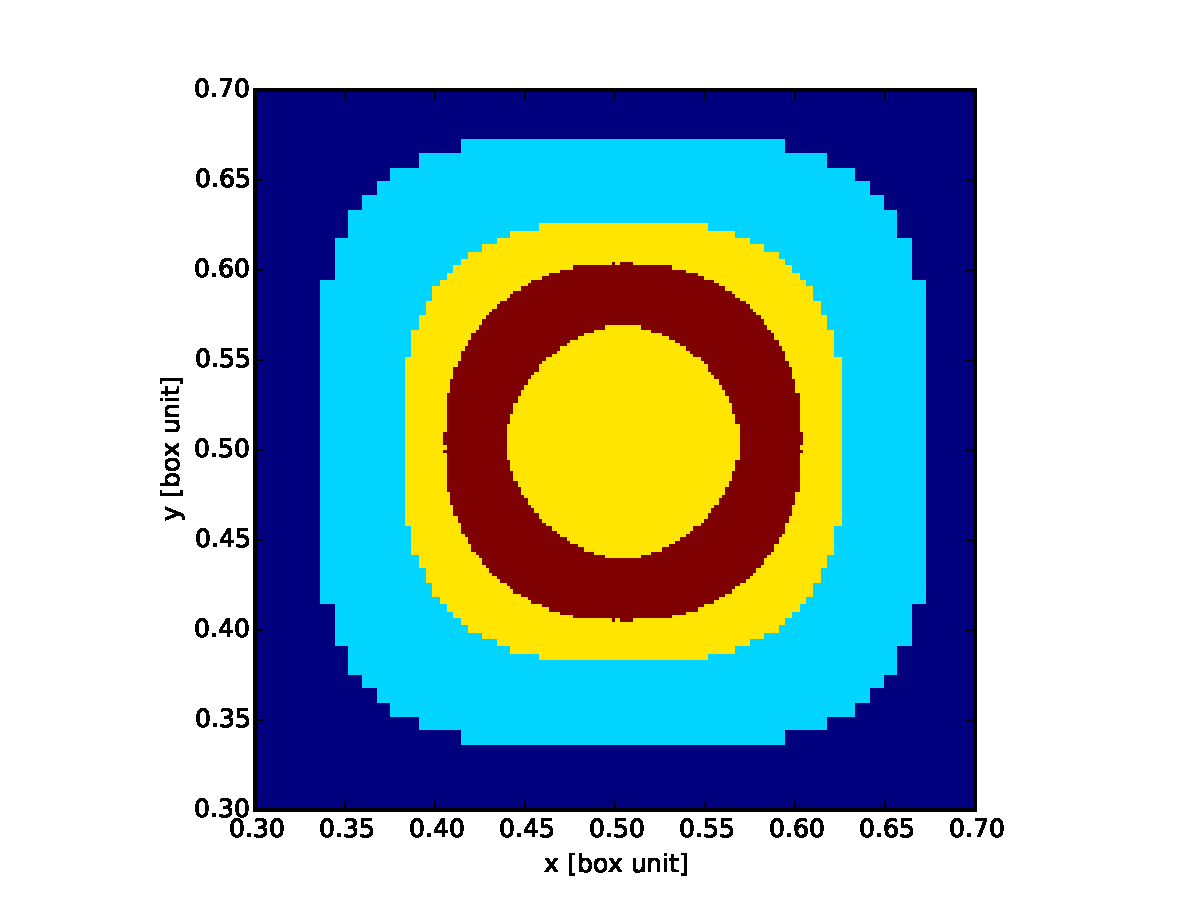
\includegraphics[width=.95\linewidth]{img/03/sedov/slice_th_1raf.pdf} 
%        \caption{Test de Sedov, raffinement (mettre la color map) }
% 		\label{fig:sedovraff}
%\end{figure}

La figure \ref{fig:sedovmethod} presente les profils obtenus a un instant donné pour les différentes méthodes d'injection d'énergie et pour les différents champs.
On observe que le front est bien situé au même endroits indépendamment de la méthode.
%Le profil de densité est présenté en échelle logarithmique pour accentuer les difference au niveau du centre. 

%\begin{figure}[htpb]
%        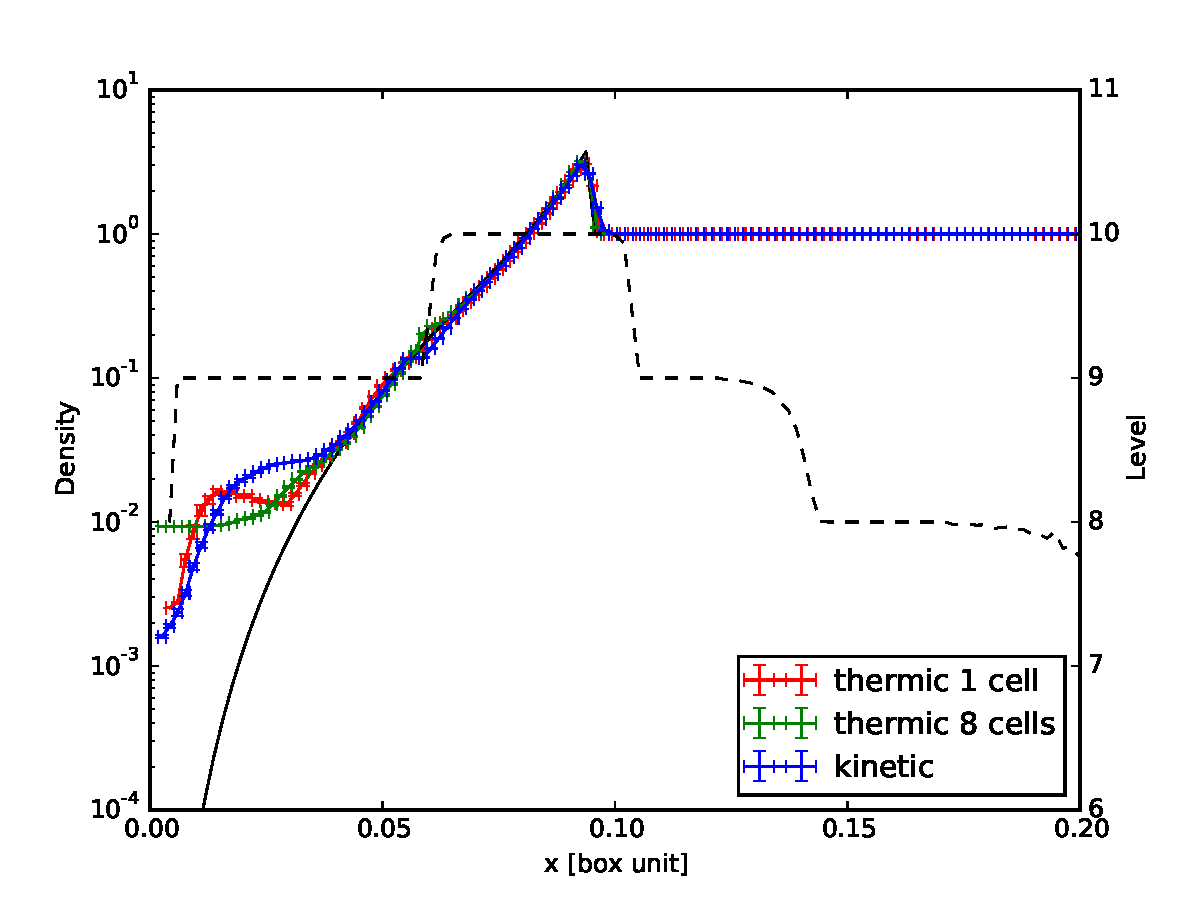
\includegraphics[height=.3\textheight]{img/03/sedov/sedov_comp_profile_den.pdf} 
%		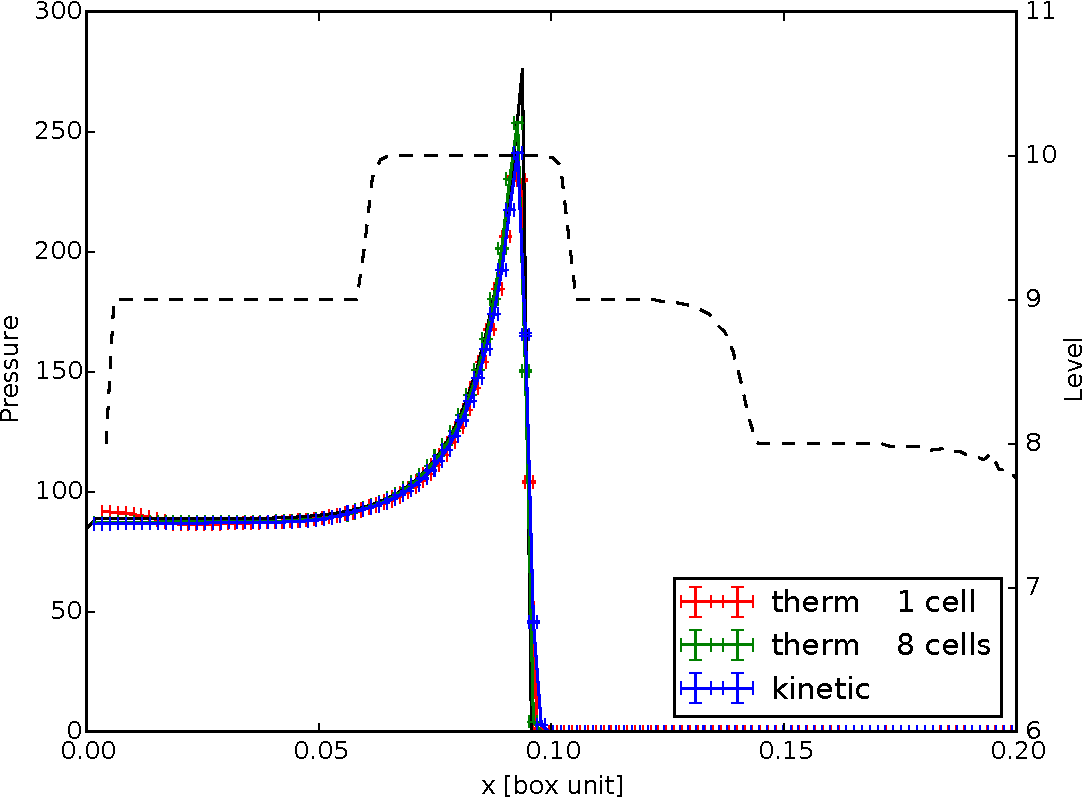
\includegraphics[height=.3\textheight]{img/03/sedov/sedov_comp_profile_pres.pdf} 
%		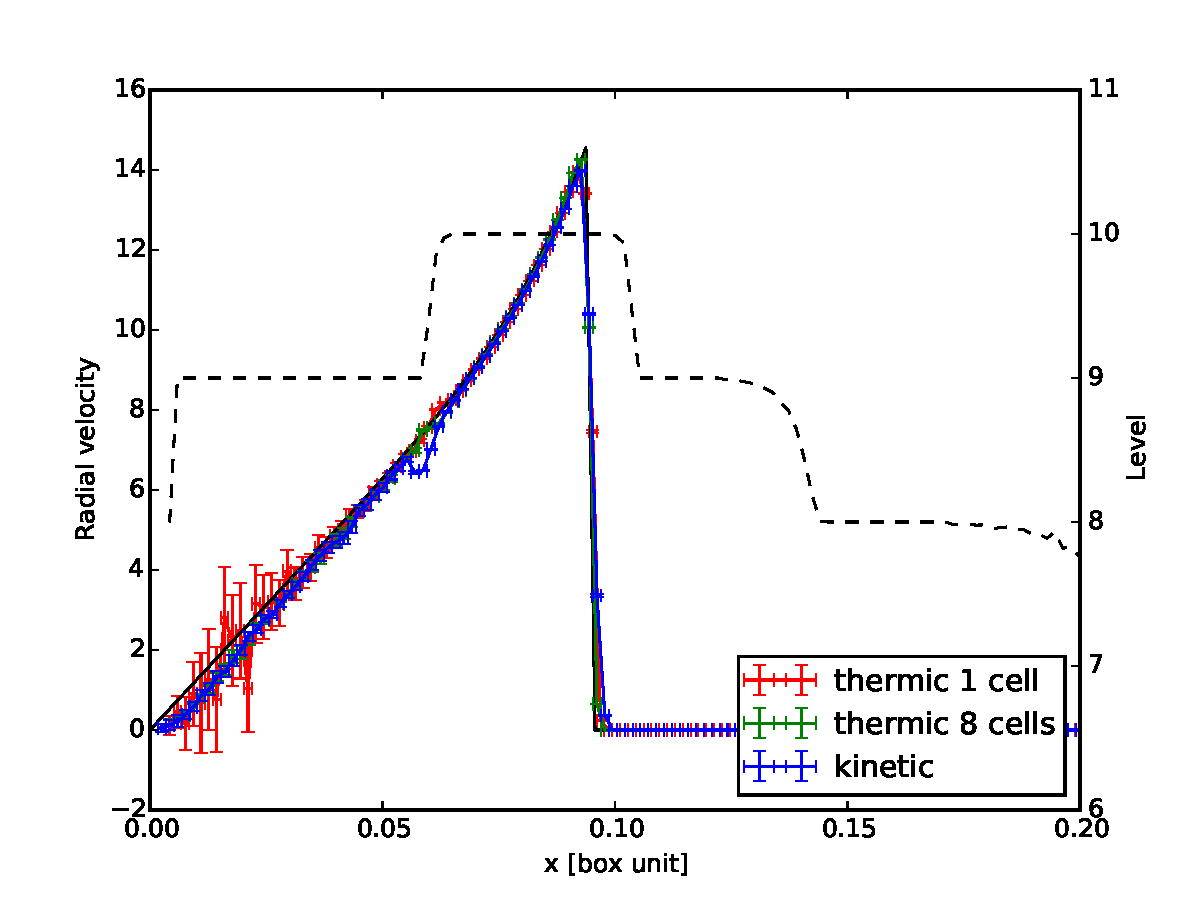
\includegraphics[height=.3\textheight]{img/03/sedov/sedov_comp_profile_vel.pdf} 
%        \caption{Test de Sedov, comparaison des profil radial en fonction des  méthodes d'injection. 
%        Densité en haut, pression au milieu et vitesse radial en bas.
%        La position et la forme du front d'onde ne dépendent pas de la méthodes d'injection utilisée.}
% 		\label{fig:sedovmethod} 
%\end{figure}


Même si les profils radiaux moyens sont comparables, on observe des différences sur la forme de l'explosion.
La figure \ref{fig:sedovslice} présente une coupe suivant l'axe z de la grille, contenant la cellule d'injection, pour les trois méthodes.
Ces différence sont dues a la grille et a la façon dont les flux sont calculés.
Dans le cas de l'injection thermique, les flux auront tendance à être suivant les axes principaux de la grille.
Ce qui donne ce motif en forme de "+" bien particulier.
Dans le cas de l'injection cinétique, les sont forcés a être dans des directions obliques, a 45°, par rapport a la l'axe de la grille.
Nous avons cette fois si une figure en forme de "x".

%\begin{figure}[htpb]
%        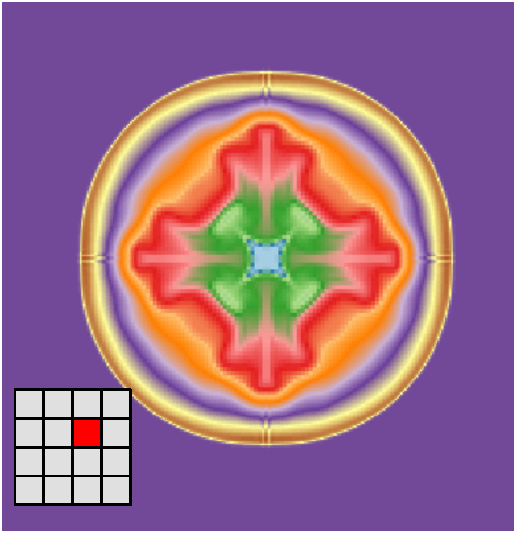
\includegraphics[height=.3\textheight]{img/03/sedov/slice_therm1.pdf} 
%		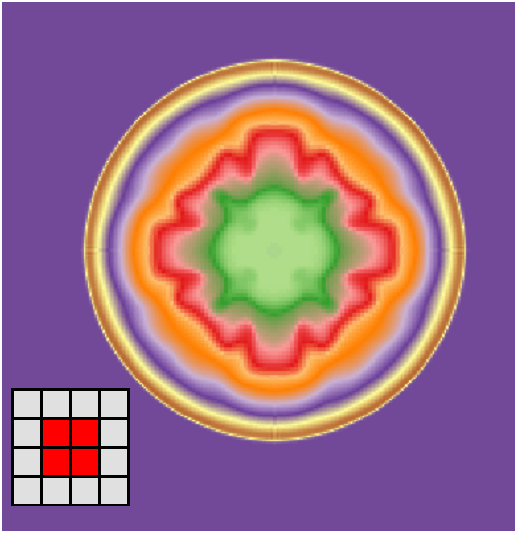
\includegraphics[height=.3\textheight]{img/03/sedov/slice_therm4.pdf} 
%		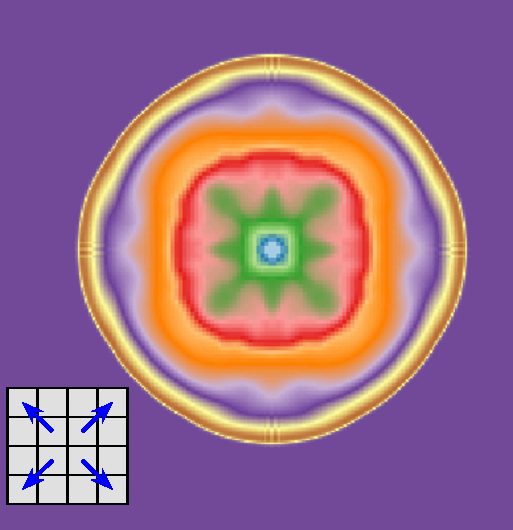
\includegraphics[height=.3\textheight]{img/03/sedov/slice_kin.pdf} 
%        \caption{Test de Sedov}
% 		\label{fig:sedovslice}
%\end{figure}



\begin{figure}[htpb]

	\centering
	\subfloat[]{        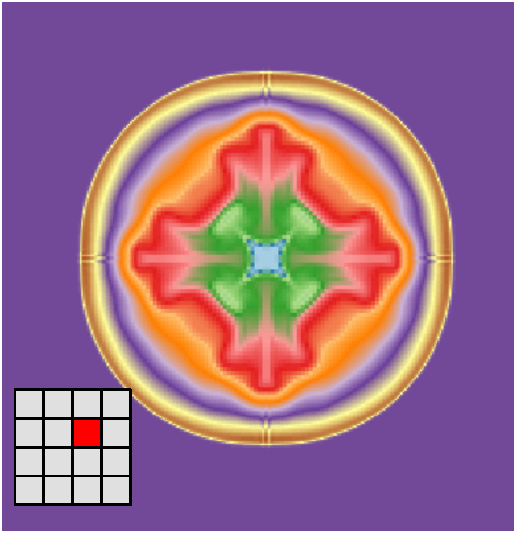
\includegraphics[width=.45\linewidth]{img/03/sedov/slice_therm1.pdf}} 
	\subfloat[]{		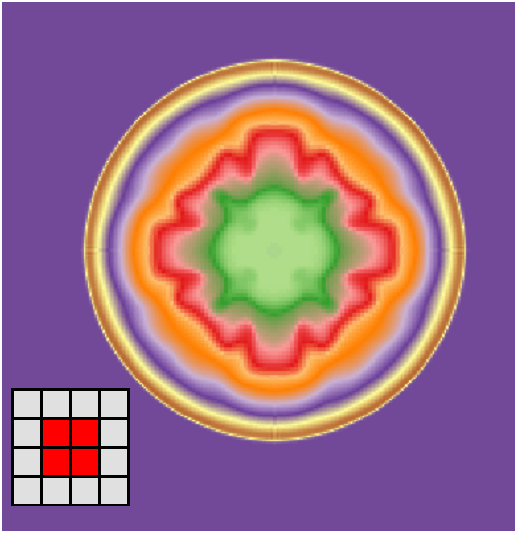
\includegraphics[width=.45\linewidth]{img/03/sedov/slice_therm4.pdf}} \\

	\subfloat[]{		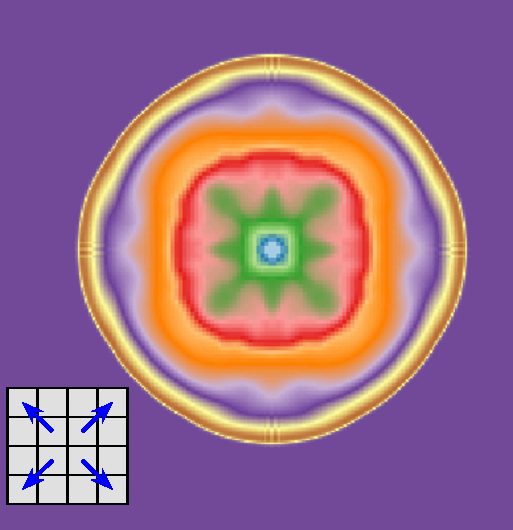
\includegraphics[width=.45\linewidth]{img/03/sedov/slice_kin.pdf} }
	\subfloat[]{		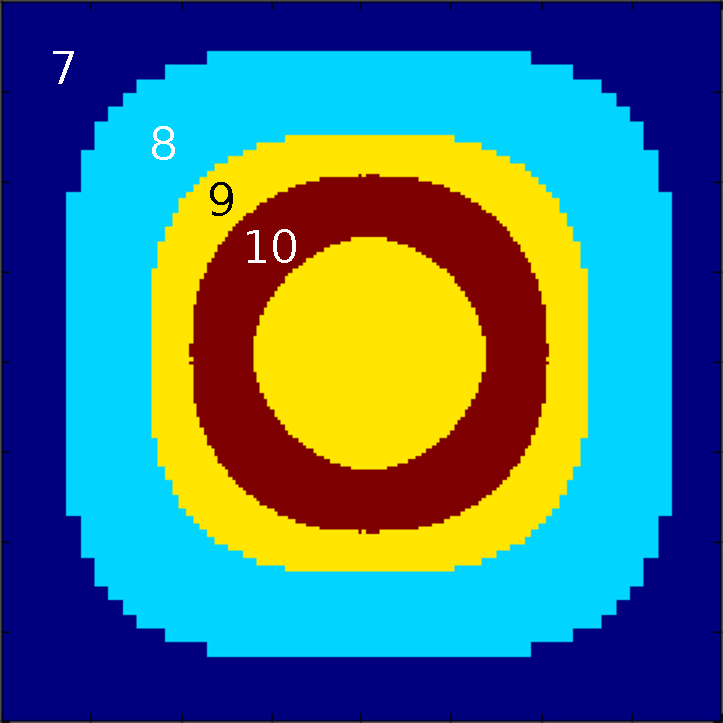
\includegraphics[width=.45\linewidth]{img/03/sedov/slice_th_1raf_cut.pdf}  }

    \caption{Différents motif d'explosion en fonction de la méthodes d'injection.
    Chaque figure représente une tranche d'une cellule d'épaisseur contenant le site de l'explosion.
    (a), (b) et (c) représente le log de la densité avec une colormap quantitative.
    A cause de la grille de calcul, il existe des axes privilégiés pour les flux, il en résulte des motif en croix et ou en losange.
    La figure (d) représente les niveaux de raffinements, le niveau 10 est aligné sur le front d'onde.
    }
 	\label{fig:sedovslice}
\end{figure}



\subsubsection{Conclusion}

La conclusion de ses tests est que les différentes méthodes d'injection sont équivalentes, au moins dans le contexte du test de Sedov.

%OK\\
%mais pas en cosmo

le pas de temps\\


\section{Tests en conditions de production}

Dans le but de tester ces différentes méthodes d'injections dans un contexte cosmologique j'ai réalisé une série de simulations.
Chacune de ces simulation est strictement identique a l'exception de la méthode d'injection d'énergie.
Les paramètres communs a toutes les simulations qui vont suivre sont les suivants:

Elles représentes un volume de 8/h cMpc cube échantillonnées par 256 cube particules de matière noire.
Ce sui mène a une résolution en masse de 3.4 10 6 M0 et une résolution spatiale de 46 ckpc sur la grille coarse.
La grille est raffinée suivant une méthode semi lagrangienne (voir Sec. \ref{sec:raffinement}).

Les condition initiales ont été générées avec MUSIC avec une cosmologie de Planck \citep{planck_collaboration_planck_2016} : 
$\Omega_m=0.3175$, 
$\Omega_v=0.6825$,
$\Omega_b=0.0490$,
$H_0=67.11$,
$\sigma_8=0.830$. 
Les simulations commences a redshift z=150.


Le premier test consiste a essayer les différents feedback avec la même quantité d'énergie injectée, et a mesurer leur impact sur la SFH cosmique.
La figure \ref{fig:sfr_methode} présente les résultats obtenus.
La méthode d'injection cinétique a plus d'impact en condition cosmologique.
Ceci est du a l'introduction de la physique du refroidissement.
La méthode thermique repose sur le principe de conversion de l'énergie interne en énergie cinétique.
La méthode thermique est connue %TODO ref
pour subir d'importante perte d'énergie.
La méthode cinétique outre passe cette conversion et mets directement le gaz en mouvement.

%TODO parler du feedback radiatif

\begin{figure}[bth]
        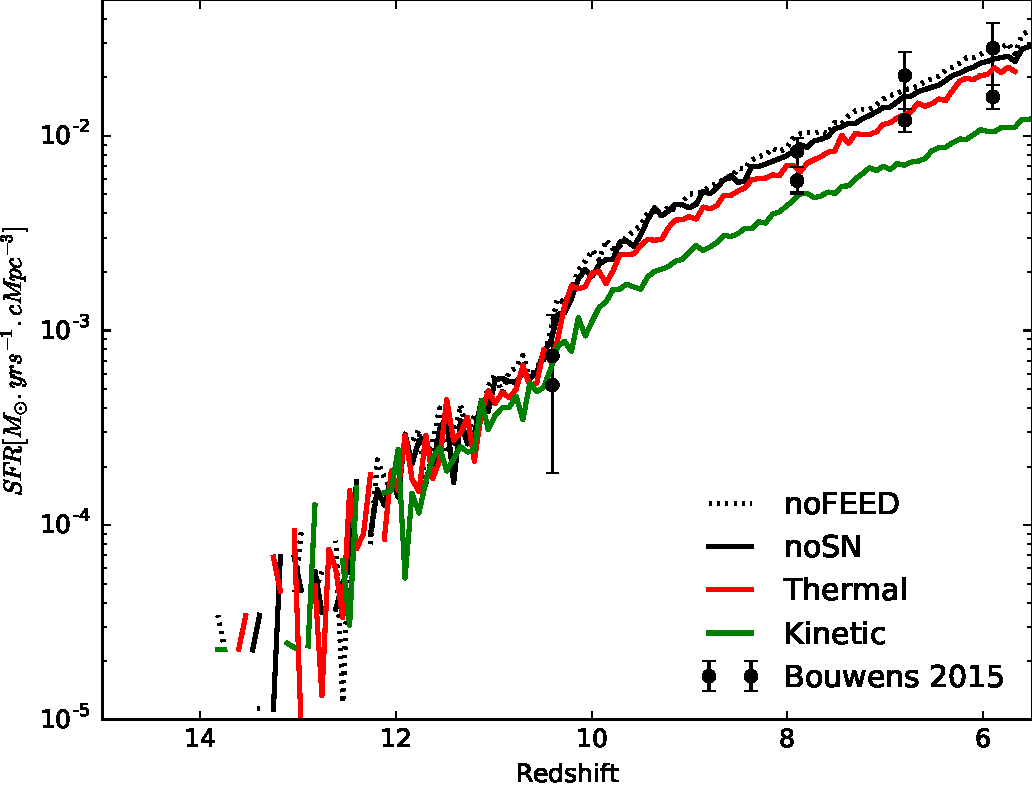
\includegraphics[width=.95\textwidth]{img/03/sedov/SFRmethode.pdf} 
        \caption{SFH cosmique en fonction de la méthode d'injection.
        Les méthodes n'impactent pas le milieu de la même manière
        }
 		\label{fig:sfr_methode}
\end{figure}

Nous aurons donc tendance préférer la méthode cinétique par la suite, vu que celle ci est plus efficace a nos échelles.
Le deuxième test consiste a utilisé la méthode cinétique et a varier la quantité d'énergie injectée.
La figure \ref{fig:sfr_egy} présente les résultats obtenus.
On y observe que plus on injecte d'énergie, plus la SFR instantanée diminue.
Ce qui est le comportement attendus puisque plus les supernovae sont puissante, plus les sur-densités de gaz sont "cassées", et donc plus difficile il devient de former de nouvelles étoiles.

\begin{figure}[bth]
        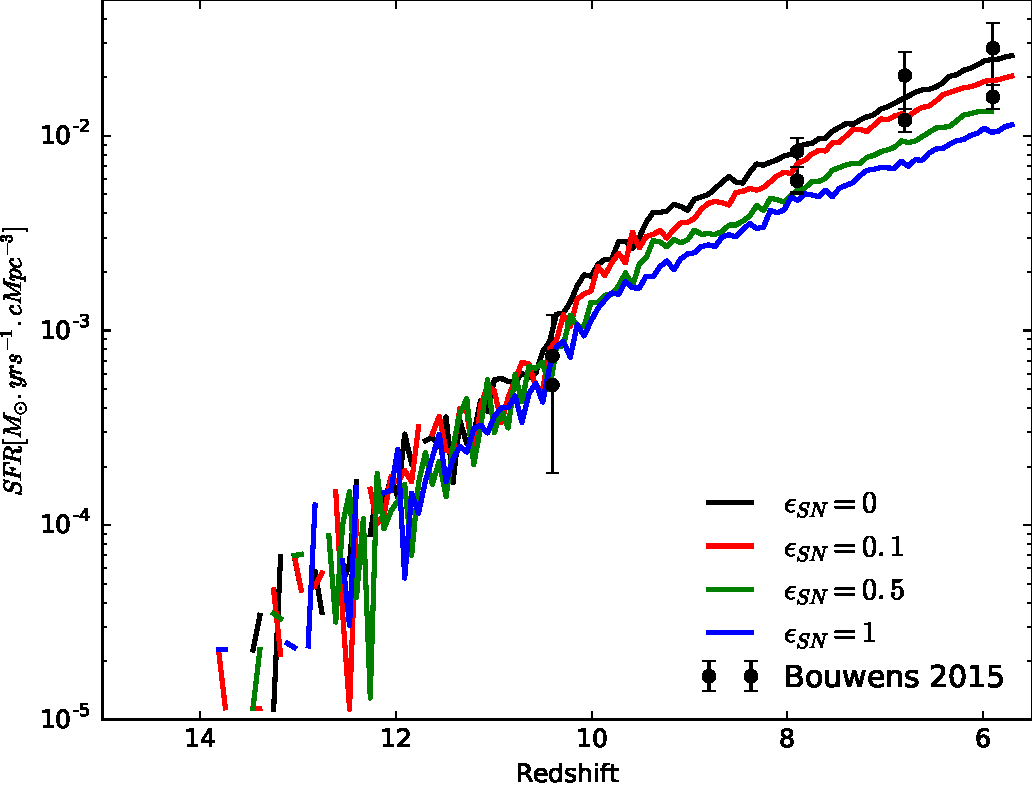
\includegraphics[width=.95\textwidth]{img/03/sedov/sneff_SFR.pdf} 
        \caption{SFH cosmique en fonction de la quantité d'énergie injectée. 
        Plus la quantité d'énergie injecté est importante, plus le taux de formation stellaire diminue.
        }
 		\label{fig:sfr_egy}
\end{figure}



Un troisième test consiste a injecter une certaine quantité d'énergie par supernovae, et a faire varier l'efficacité de formation stellaire.
En effet plus on forme d'étoiles et plus le feedback devient important, mais plus il y a de feedback, moins il est facile de former de nouvelles étoiles.
Le couplage entre feedback et formation stellaire n'est pas clair et mérite d'être exploré.
La figure \ref{fig:sfr_sfe} présente ce test pour trois efficacité de formation stellaire avec un modèle de feedback cinétique et une efficacité de supernovae de 100 \%.
On observe un fort couplage entre feedback et formation stellaire, a tel point que pour une efficacité de formation stellaire de 10\% le feedback mène a une SFH décroissante.

\begin{figure}[bth]
        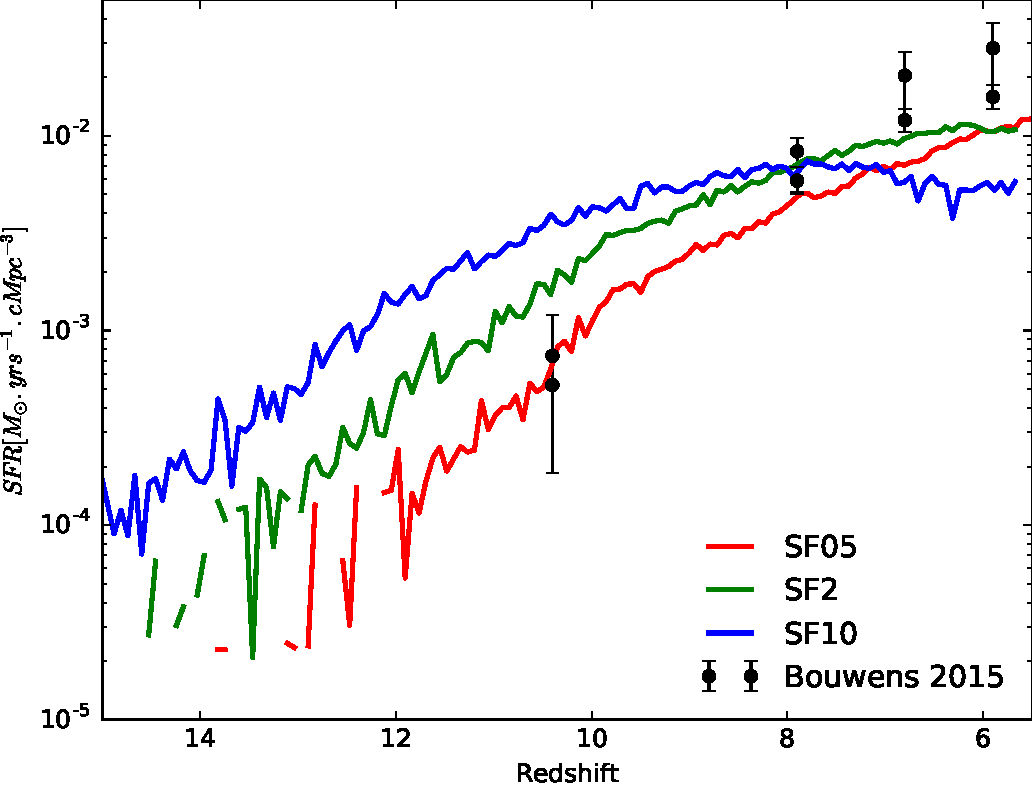
\includegraphics[width=.95\textwidth]{img/03/sedov/SFR_sfeff.pdf} 
        \caption{SFH cosmique en fonction de l'efficacité de formation stellaire.
        Toutes les simulation utilise la même méthode d'injection et la même quantité d'énergie.
		L'effet du couplage est bien présent.
        }
 		\label{fig:sfr_sfe}
\end{figure}

Une observation importante par rapport au deuxième test est qu’indépendamment de la quantité d'énergie injectée, et que même si la SFR est significativement impacté, l'histoire d'ionisation reste quasiment constante (cd fig \ref{fig:xion_sneff}).


\begin{figure}[bth]
        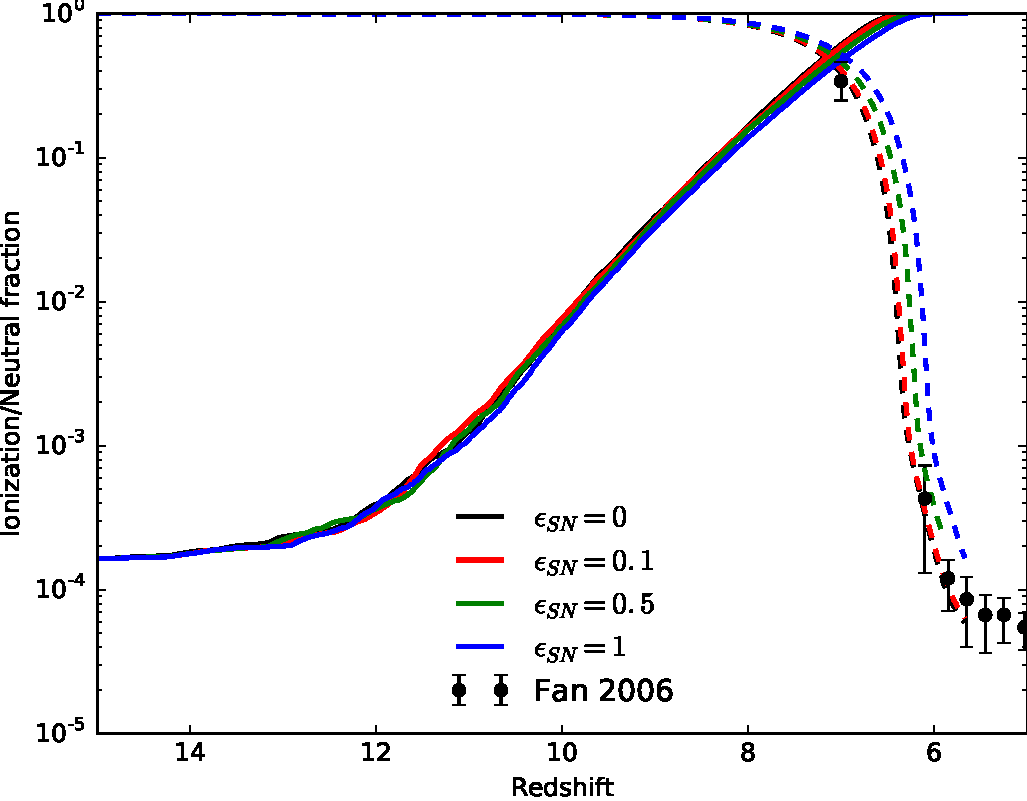
\includegraphics[width=.95\textwidth]{img/03/sneff_xion.pdf} 
        \caption{Malgré une SFH différente (voir figure \ref{fig:sfr_egy}), l'histoire d'ionisation est conservée en changeant la quantité d'énergie injectée.
        }
 		\label{fig:xion_sneff}
\end{figure}

Cet effet est inattendu car si la quantité d'étoiles diminue, la quantité de radiation diminue d'autant, et donc la fonction d'ionisation globale devrait être impacté.
Or ce n'est pas ce qui est observé ici.
Dans le but d'explorer cet effet, nous allons nous concentrer dans la suite a une étude galaxies par galaxies.













